%
%	overview.tex
%
%	Project Details: Overview
%
%	John Hughes and Michael Jean
%	University of Manitoba
%

\section{Overview and Goals}

The Formula SAE vehicle is a performance car built with the primary goal of doing well in the 
dynamic events at the yearly competitions. These events test the vehicles abilities in acceleration, 
braking, and handling.

The vehicle as a whole is primarily a mechanical device, but carries several critical electronic 
control systems. Three key mechanical systems that either require electronic control or can benefit 
from electronic control are

\begin{itemize}
\item the \emph{internal combustion engine} (ICE\nomenclature{ICE}{Internal Combustion Engine}); 
\item the \emph{braking system}; and
\item the \emph{suspension system}.
\end{itemize}

\subsection{Internal Combustion Engine}

\nomenclature{MAP}{Manifold Absolute Pressure}
\nomenclature{ECU}{Engine Control Unit}
\nomenclature{DAQ}{Data Aquisition device, provides and logs high-performance GPS, accelerometer, and ADC input data}
\nomenclature{GPS}{Global Positioning System}

The ICE is a \emph{Honda CBR600F4i}, a 600 cm$^3$ super-sport class engine with an internal 6-speed 
chain driven transmission. 

The engine has a set of sensors attached to it, including

\begin{itemize}
\item an O$_{2}$ sensor;
\item a Manifold Absolute Pressure (MAP) sensor; 
\item an oil pressure sensor;
\item a water temperature sensor;
\item a throttle position sensor;
\item a gear position sensor;
\item cam and crank position sensors; and
\item wheel speed sensors.
\end{itemize}

Several tasks and responsibilites are best accomplished by electronic means, i.e.,

\begin{itemize}
\item the fuel injectors must be provided with timing signals;
\item the spark coils must be provided with firing signals;
\item a signal to engage the starter solenoid must be provided;
\item the clutch and gear selection levers must be intelligently actuated to change gears; 
\item the clutch must be intelligently actuated to enable the vehicle to move forward slowly;
\item the intake plenum valve must be opened or closed as driving conditions warrant; and
\item sensor outputs must be logged and relayed to team members wirelessly.
\end{itemize}

A specialized third-party component called the \emph{Engine Control Unit} (ECU) acts as a 
closed-loop feedback system that controls the fuel injector and spark coil systems that
in turn control the combustion cycle of the engine. The particular model of ECU used by the 
Formula SAE car is the S80Pro from DTAFast \cite{s60pro}. The ECU reads O$_{2}$ and MAP sensor
outputs and adjusts fuel injector and spark coil timings to keep the engine running smoothly. 
The ECU also features a traction control system that monitors wheel slip and cuts spark signal 
to help give traction when one of the drive wheels is slipping. The ECU collects the various sensor 
readings and makes them available through electronic data buses at a fixed frequency. 

\begin{figure}[H]
	\centering
	 	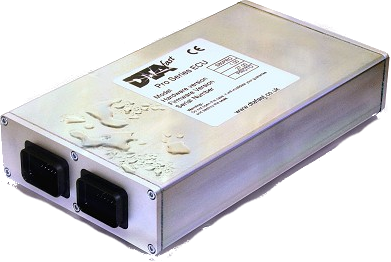
\includegraphics[scale=0.5]{figures/s80.png}
    \caption{DTAFast S80Pro Engine Control Unit (ECU)}
    \label{fig:s80pro_product}
\end{figure}

The ICE is started by energizing a \emph{starter solenoid}. This solenoid relays a large electric 
current to the \emph{starter motor}, which turns over the engine and causes it to start. An 
external control signal from the driver must engage and disengage the starter solenoid.

The ICE has an internal 6-speed manual transmission. The first, fifth, and sixth gears have been 
removed to reduce weight. The vehicle is not operated at speeds that would benefit from the presence 
of the fifth or sixth gear, and launching from second gear provides the best acceleration. 

A pre-tensioned spring lever controls the clutch. The spring keeps the clutch engaged when there is 
no force on the lever. As force is applied to the lever, the clutch is gradually disengaged. The 
relationship between lever position the distance between the clutch plate and flywheel is non-linear. 

Another pre-tensioned spring lever controls the gear selection. The gear selector may be rotated in 
either direction from its rest point. Up-shifting is accomplished by rotating the lever in one 
direction, while down-shifting is accomplished by rotating the lever in the opposite direction. 

Opearting a purely mechanical manual transmission is taxing on the driver. Ideally, shifting
between gears should happen as quickly as possible, with the least amount of driver focus. 
Engaging of the clutch should be as smooth as possible. 

The intake plenum valve controls the effective length of the manifold and therefore the mass air
flow in the engine. Engine performance is directly affected by the amount of air available for
combustion. 

Another specialized third-part component called the \emph{Data Aquisition Device} (DAQ) is used
to log and relay sensor data to other electronic devices.

The particular DAQ used is the model DL1 from Race Technology \cite{DL1Dsheet}. The DL1 is an 
expandable data logger with built-in 20-Hz GPS and 3-axis accelerometer. Race Technology provides 
a software suite that communicates with the DAQ using a documented serial protocol. Every item that 
the DAQ logs is output to its own channel in real time on the serial bus. It is also possible to 
configure the software to recognize new channels for arbitrary types of data. 

\begin{figure}[H]
	\centering
	 	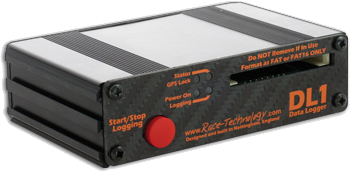
\includegraphics[scale=0.5]{figures/dl1.png}
    \caption{Race Systems DL1 Data Acquisition Device (DAQ)}
    \label{fig:dl1_product}
\end{figure}

\subsection{Braking System}



\subsection{Suspension System}
